\documentclass{article}

\usepackage{amsmath}
\usepackage{fancyhdr}
\usepackage{graphicx}
\graphicspath{{}}

%% some colours
\usepackage{color}
\definecolor{deepblue}{rgb}{0,0,0.5}
\definecolor{deepred}{rgb}{0.6,0,0}
\definecolor{deepgreen}{rgb}{0,0.5,0}
\definecolor{backcolour}{rgb}{0.95,0.96,0.93}

%%%%%%%%%%%%%% CODE STUFF %%%%%%%%%%%%%%
%%%%%%%%%%%%%%%%%%%%%%%%%%%%%%%%%%%%%%%%
\usepackage{cprotect} % to be used in sol
\usepackage{listings} % for code display
% setting code style
\newcommand\pythonstyle{\lstset{
        language=Python,
        backgroundcolor=\color{backcolour},
		basicstyle=\footnotesize,
		otherkeywords={self},
		keywordstyle=\footnotesize\color{deepblue},
		emph={__init__},
		emphstyle=\footnotesize\color{deepred},
		stringstyle=\color{deepgreen},
		frame=single,
		showstringspaces=false  ,
		breaklines=true,
		numbers=left,
		numberstyle=\footnotesize,
		tabsize=4,
		breakatwhitespace=false
	}}

% Python environment
\lstnewenvironment{python}[1][]{
    \pythonstyle
    \lstset{#1}
}{}

% Python for external files
\newcommand\pythonexternal[2][]{{
    \pythonstyle
    \lstinputlisting[#1]{#2}
}}

% Python for inline
\newcommand\pythoninline[1]{{\pythonstyle\lstinline!#1!}}

%%%%%%%%%%%%%%%%%%%%%%%%%%%%%%%%%%%%%%%%
% setting the style for ex documents
\pagestyle{fancy}
\fancyhf{}
\fancyhead[L]{\thetitle}
\fancyhead[C]{}
\fancyhead[R]{\theauthor}
\renewcommand{\headrulewidth}{0.4pt} %obere Trennlinie
\fancyfoot[L]{Due: \thedate}
\fancyfoot[R]{\thepage} %Seitennummer
\renewcommand{\footrulewidth}{0.4pt}

% include solutions
\newcommand\sol[1]{{\large\textbf{\\Solution:}}#1}
\usepackage{setspace}

\title{BPP Exercise 11 - NumPy and Matplotlib}
\author{A. Hain, M. Nipshagen}
\date{18.06.2018, 10:00}


\makeatletter
\let\thetitle\@title
\let\theauthor\@author
\let\thedate\@date
\makeatother


\newcommand\itemsub[1]{
	\begin{itemize}
		\item #1
	\end{itemize}
}

% do not include solutions
\renewcommand\sol[1]{}


\begin{document}

The deadline for this exercise sheet is \textbf{Monday, \thedate.}

\section*{Introductory Words}
Remember that you need proper documentation to pass
the homework. The documentation doesn't need to be \textit{perfect}, but
everything that needs a docstring, should have a docstring.\\

\noindent Please make sure that your libraries are up to date. For numpy your
version must be $\geq$ 1.13 and for matplotlib $\geq$ 2.2. You can check the
installed version either using pip: \verb|pip show numpy matplotlib| or
directly in Python:
\begin{python}
import numpy as np
import matplotlib as mpl

print("Numpy:", np.__version__)
print("Matplotlib:", mpl.__version__)
\end{python}
If you need to upgrade either, use conda or pip: 
\verb|conda install numpy matplotlib| or \verb|pip install numpy matplotlib|.
This should install the latest version.

\section{Warm-Up}
\subsection{Number Stuff with NumPy}
Given the following ndarrays:
\begin{python}
import numpy as np


a = np.array([1, 2, 3])
b = np.array([-1, 2, -3])
c = np.arange(1, 10).reshape(3,3)
d = np.array([[1,2],[-2,-1],[5,5]])
\end{python}
calculate the following operations. Order matters.
\begin{itemize}
	\item The dot product of a and b
	\sol{\pythoninline{np.dot(a, b)}}
	\item The dot product of c and a
	\sol{\pythoninline{np.dot(c, a)}}
	\item The matrix multiplicative of c and d
	\sol{\pythoninline{np.matmul(c,d)}}
	\item The matrix multiplicative of the transpose of d and c
	\sol{\pythoninline{np.matmul(d.T, c.T)}}
	\item the overall mean of a and b together
	\sol{\pythoninline{np.mean([a,b])}}
\end{itemize}

\subsection{Plot, plot away}
\subsubsection{Crossed out}
Plot the following functions from $-4$ to $8$ into one figure.
Use at least 100 points.\\
\emph{Note:} You only need to create \textit{one} ndarray for the x-coordinates.
\begin{itemize}
	\item $y_1 = 2x - 2$
	\item $y_2 = -2x + 6$
	\item $y_3 = 0.25(x - 2)^2 + 2$
	\item $y_4 = -0.25(x - 2)^2 + 2$
\end{itemize}

\subsubsection{Markers all around}
From NumPy's random module use the normal function to create 1000 randomly
drawn numbers. Draw from a normal distribution with center (loc) 0 and a
standard deviation (scale) of 5. Then plot those numbers into a histogram,
with 25 bins, and a bar width of 0.9.\\
Have a look at the numpy documentation for 
\href{https://docs.scipy.org/doc/numpy/reference/generated/numpy.random.normal.html#numpy.random.normal}{random.normal}.

\subsubsection{Who is that plot?!}
In the accompanying .zip archive you can find the \verb|plot_me| module. 
Import the \verb|get_x_y| function from it. The function will return two
numpy ndarrays in the form \verb|x, y|, which are x and y coordinate pairs.
Plot those pairs using a scatter plot, with a scale (\verb|s|) of 0.5.\\
\emph{Note:} The function can take a few seconds to compute.


\section{The great Plotting}
\subsection{Wavy Waves}
Using your new gained knowledge, recreate the figure in the image  
below \ref{fig:sines}.\\
The graphs are plotted from $-2\pi$ to $2\pi$. You do not have to modify
the ticks on the x-axis. If you want to recreate those as well, look into
\href{https://matplotlib.org/api/_as_gen/matplotlib.pyplot.rc.html}{the rc doc},
which allows you to set all kind of formatting. Especially interesting is the 
\texttt{usetex} boolean property of \texttt{text}. Also see
\href{https://matplotlib.org/users/usetex.html}{this explanation}.

\begin{figure}[h!]
	\makebox[\textwidth][c]{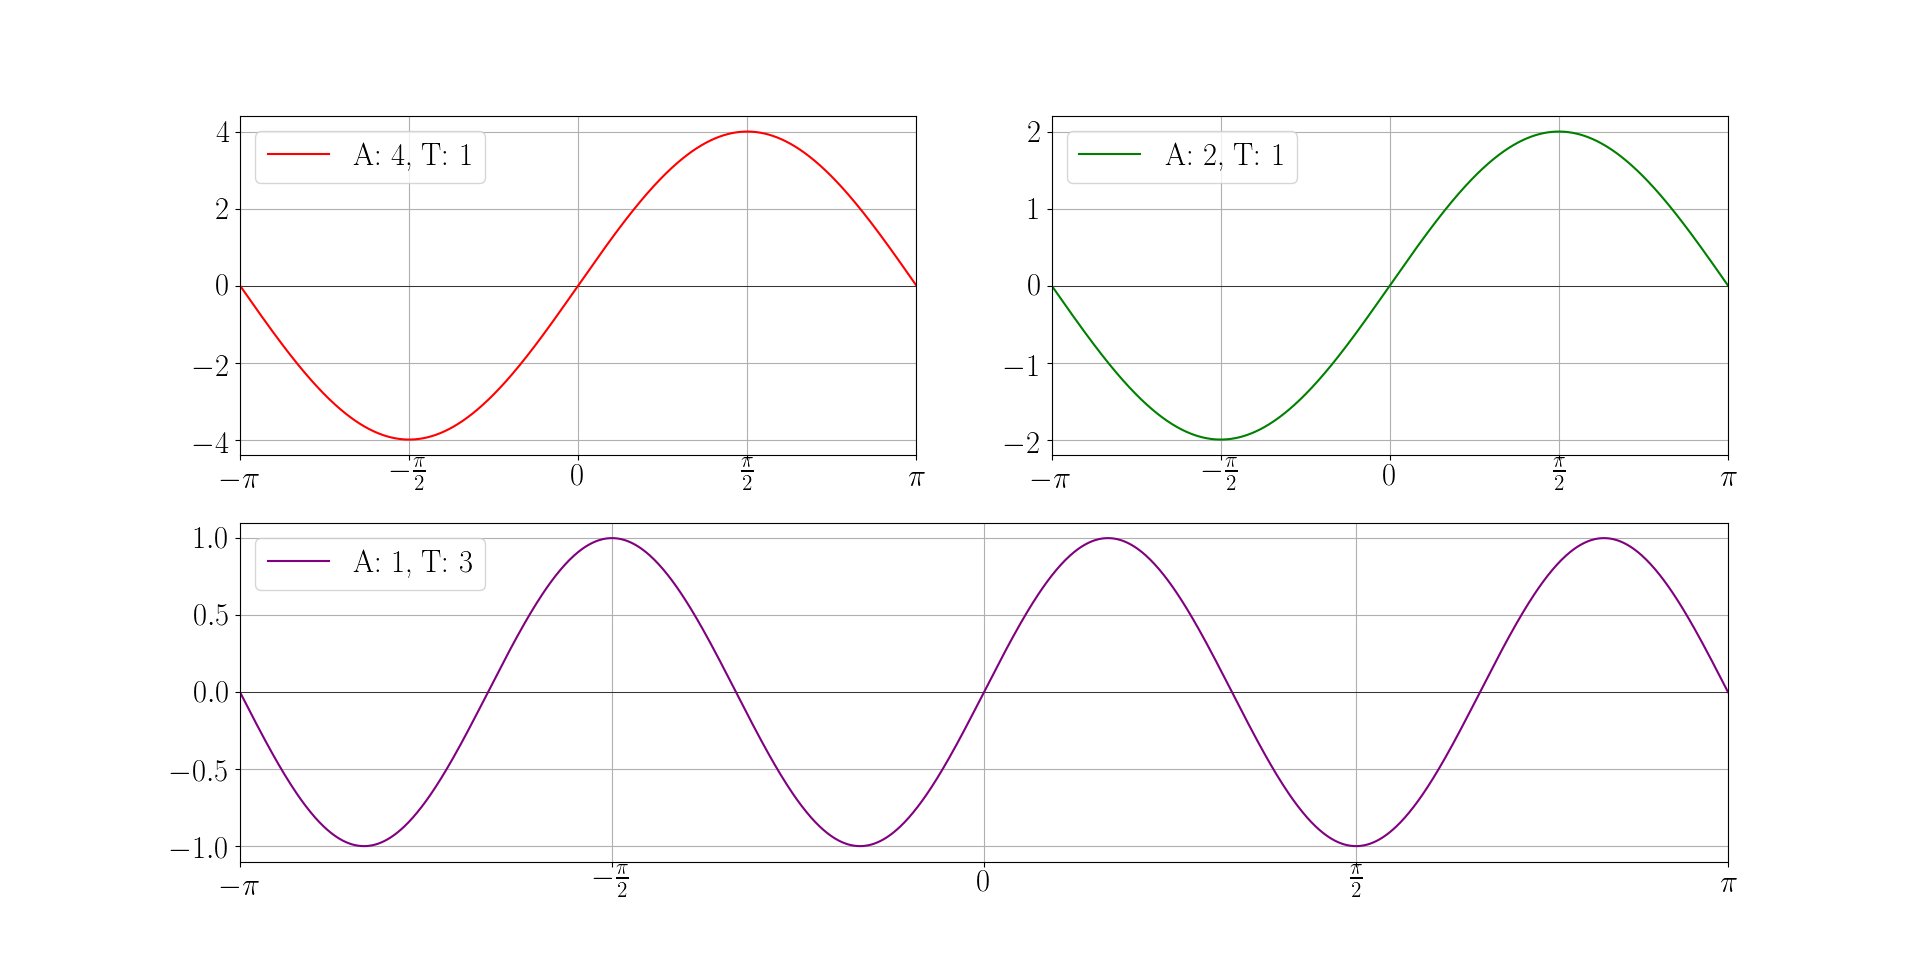
\includegraphics[width=1.5\textwidth]{sines}}
	\caption{Three sine waves with different properties}
	\label{fig:sines}
\end{figure}

\subsection{Bonus: All alive.}
Let's bring this plot to life! Animate the sine waves in such a way, that
the top left sine wave moves to the left and the top right sine wave moves
to the right. Wave-y!
\subsection{Bonus-Bonus: Wave the wave}
Now that we got that animation up and going, let's animate the bottom sine
wave as well. This time not just left and right, but up and down as well.
Move the whole sine wave on a sine wave. So that the whole curve shifts to
the left as well as up and down as if it was moving along another sine wave.\\
This is a tricky one.

\end{document}
